\documentclass[main.tex]{subfiles}

\begin{document}
\chapter{Concept Design}
\chaplabel{conceptDesign}

\section{Platform Selection}
A platform is used as a means to mount the required detection equipment and to act as the foundation for a completely autonomous system.  Design and construction of the platform is not in the scope of the project and so the modification of an existing platform was the preferred approach. The selected platforms included in the decision process were based directly on their availability to the project, whether a commercial product or the loan of equipment. Primary factors that were considered during the selection process were taken from the Project Specifications (see \secref{performance}) and the Project Scope (see \secref{projectScope}). The following list outlines the criterion used during the process and the decision matrix (\figref{platformDecision}). In general, a score of 5 indicated that a requirement had only just been satisfied or that the criterion was only just feasible for that platform, with any difference being representative of a rise or fall in the platforms capability with respect to that requirement. Scores had a lower limit of 1 and an upper limit of 10.
\begin{itemize}
\item Cost: Based on a budget of \$16,500. A platform cost nearing \$5,000 indicated that the requirement had been met. A score of 10 indicates platform supplied in-kind and 1 indicates financially infeasible.
\item Implementation of Auto-Control: How involved the process of implementing the direct hardware required for remote operation would be. A low score indicates a difficult process with many sub-systems, whereas a high score indicates little to no work necessary. Requirement was met if implementation of hardware was a feasible task.
\item Control/Manoeuvrability: How appropriate the platform was expected to be regarding manoeuvrability assuming auto-control was implemented successfully. This included speed, acceleration, turn radius, and stopping distance.
\item Implementation of detection equipment: Ease of installation of detection equipment and expected effectiveness of the platform and sensor combination from a landmine detection point of view.
\item Payload: Platform's ability to support the required 100 kg payload.
\item Terrain Traversing: How capable the platform is at traversing the required terrain. This includes dry and loose sand or gravel with minimum obstacles and a 15 degree gradient.
\item Portability: Level of portability. A higher score indicates simpler transport with less disassembly required. The requirement had been satisfied if transport was possible in the back of a ute or trailer.
\item Operation Time: {\color{red}{need something here, i dont think theres anything in requirements for it yet}}
\item Navigation: How direct and efficient the path of the platform for mine-detecting purposes was expected to be. This involves aspects such as duration and tightness of turns and mine avoidance techniques.
\end{itemize}

\begin{figure}[ht]
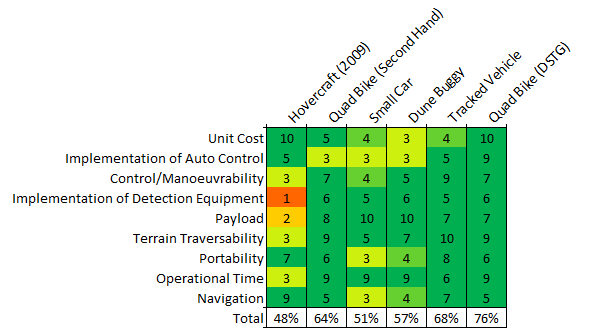
\includegraphics{4-ConceptDesign/platformDecision.png}
\centering
\caption{Platform Decision Matrix} \figlabel{platformDecision}
\end{figure}

\Figref{platformDecision} summarises each of the \sout{available}\textcolor{green}{considered} platforms which are detailed further in following subsections. If a criterion is met with a score of 5 or higher it is coloured green, otherwise the colour transitions to red - a score of 1. \textcolor{green}{This color scale seems awfully arbitrary. Why max out at 5? It's a pretty small detail to get nitpicky over but I don't think the chart is as clear as it could be.} It was evident that the hovercraft did not meet majority of the requirements to be the supporting platform. Commercial quad bikes, small cars, or dune buggies could have been used with some modifications to the structure, however a tracked vehicle or the quad bike offered by DSTG were clearly the two best options.

The DSTG quad bike was selected over a tracked vehicle for a number of reasons. These included direct availability, financial restrictions, and the completed state of auto control hardware already on the quad bike.

\subsection{Hovercraft}
Access was made available to an existing hovercraft from a 2009 Adelaide University Honours Project. Analysis of the technical report \parencite{hovercraft2009} and practical and theoretical evaluations showed that the lift fan was able to support a payload of up to 22 kg and the thrust fans were only just capable of moving the craft on a flat, smooth surface. For complete automation only actuators for the lift motor would be required as remote operation for the thrust system had already been implemented. The stopping distance is lacking due to the time required to rotate fans for reverse thrust. The hovercraft has an advantage over other platforms through its ability to pass directly over a mine without detonation occurring, however, this 'sliding' advantage introduces new problems when developing a path tracking algorithm due to the advanced dynamics of the platform. The purchasing of a recreational hovercraft more suited to the requirements would not have been financially feasible. Through verbal discussion with DSTG, it was revealed that vibrations produced through the lift and thrust systems on hovercraft platforms were detrimental to the effectiveness of the sensor equipment. Thus, the DSTG has advised against the use of a hovercraft as the platform for mine-detecting purposes.
\begin{figure}[ht]
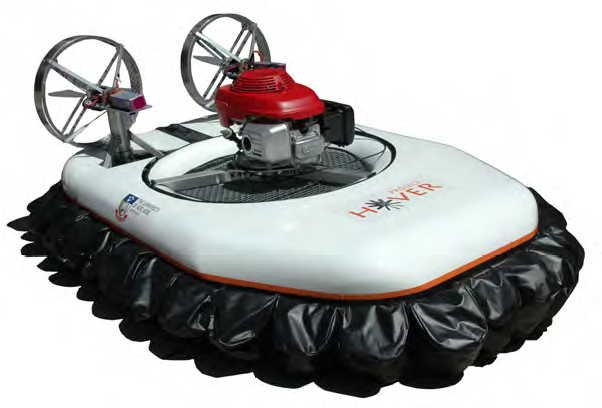
\includegraphics[width=0.4\textwidth]{4-ConceptDesign/HovercraftPic.png}
\centering
\caption[2009 Adelaide University Honours Project Hovercraft]{2009 Adelaide University Honours Project Hovercraft \parencite{hovercraft2009}} \figlabel{hovercraftPic}
\end{figure}

\subsection{Quad Bike}
Quad bikes are designed as all terrain vehicles and are capable of traversing even the most demanding terrains. Utility quad bikes are intended to carry large loads as well as a human operator and so load limits are frequently larger than 100 kg. Due to the nature of the platform and through visual inspection, mounting points for sensor brackets and electronic systems are located in various positions.  Environmental conditions are of little concern to this platform which will be encountered and traversed with ease for ranges of over 100 km. Turning radius for quad bikes are typically in the range of 3-4 metres.
The DSTG have offered the use of one of their autonomous quad bikes to be used as the platform. The DSTG quad bike is a Honda TRX450r and has a weight load capacity of 110 kg. The quad bike has been previously fitted with remote control capabilities and is in good working condition, however \textcite{scheiner2011} recommended that the brake actuator be replaced as well as some electronics. As the platform already has remote control capabilities, transport becomes a much easier task especially with a trailer or ute with a ramp.
\begin{figure}[ht]
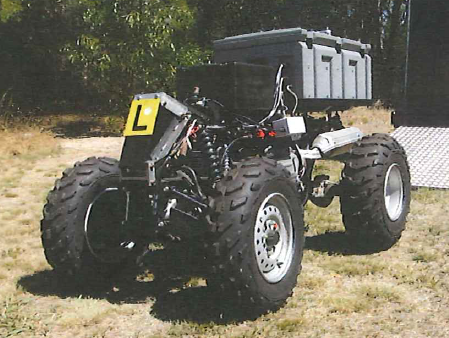
\includegraphics[width=0.4\textwidth]{4-ConceptDesign/2011quadbike.PNG}
\centering
\caption[DSTG Autonomous Quad Bike]{DSTG Autonomous Quad Bike \parencite{scheiner2011}} \figlabel{2011quadbike}
\end{figure}

\subsection{Small Car ?}
turn radius' of around 30 feet.

\subsection{Dune Buggy ?}

\subsection{Tracked Vehicle}

\section{Navigation}
The navigation system is responsible for communicating to the quad bike two primary functions, how to follow a low curvature path and how to turn a specified angle. Platform navigation will be primarily handled via waypoints. After a region is selected by a user it is broken down into a series of waypoints which, once connected, will form a path for the quad bike. In the alternate use case, the navigation system will operate based directly on waypoints created from a user defined path.
\subsection{Path Tracking}
\Textcite{snider2009} provides an empirical comparison of path following algorithms and is shown in \figref{trackingComparison}. Tracking Methods are ordered by implementation difficulty from least difficult to most difficult.\\
\textcolor{red}{This figure 4.4 one is an issue since the writing is smaller than our font. Either find a new comparison or redo it with larger text or better colours... :/}
\begin{figure}[ht]
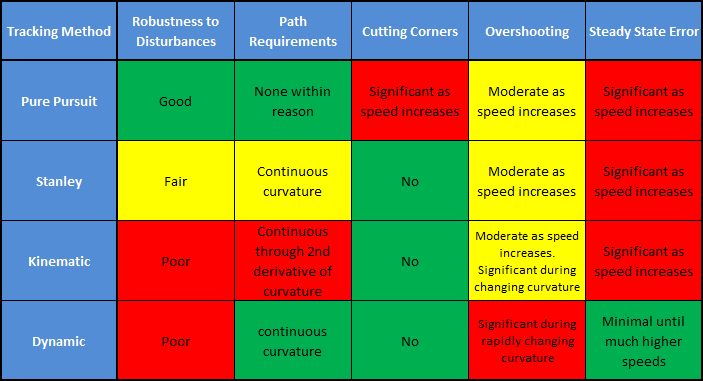
\includegraphics[width = \textwidth]{4-ConceptDesign/pathTrackingSummary2.png}
\centering
\caption{Empirical Comparison of Path Tracking Algorithms \parencite{snider2009}} \figlabel{trackingComparison}
\end{figure}
\subsection{Turning the Platform a Specified Angle}
At the end of a swathe the platform will be required to turn a specified angle within a small area defined by the width of the sensing arrays. Alternatively, if the scan history is available to the platform in the form of a map a larger area may be available to conduct the turn. Due to little or no literature on the unique topic an adaptation of the simplified Ackermann model and path tracking algorithms will be used to achieve the turn.

\section{Signal Processing}
\seclabel{signalconcept}
\textcolor{red}{Jono, might be good to cover this section for some of the concept designs for the code}

As noted in \secref{gpr}, the detection depth and resolution are generally fixed parameters of the transmitting and receiving antennas of the physical device. The signal processing software will be designed to operate effectively on the hardware available, which is the GPR unit supplied to the project courtesy of the DSTG. The model supplied is a single GPR (non-array) unit with three interchangeable antennas which allow the selection of transmission and receiving frequency. The three heads supplied are:
\begin{itemize}
\item 800 MHz
\item 1.4 GHz
\item 2.0 GHz
\end{itemize}
During the course of the project a single antenna head will be used, determined by initial testing to be the frequency which generates the highest resolution data while providing depth of scanning as required by the project goals. A suitable metal detecting unit will be sourced from commercially available systems to match the detection range of the GPR unit supplied, to provide the greatest overlap of scanning capacity.
The software and systems developed will be generated as a proof-of-concept using the initial available equipment, with considerations made to allow for simple expansion to array based detectors for the benefits discussed in \secref{gpr}. 

In consideration of the project timeframe and expected capacity of group members, the proposed signal processing system will seek to employ a Decision-level Sensor Fusion strategy to improve the detection and false-positive error rates over that of the individual sensors. This is expected to be achieveable and will demonstrate the core abilities of the sensor fusion strategy to improve detector classification. \\

The decision-level sensor fusion becomes more accurate with more decision metrics available about the object. To make the most of the sensors available to the platform, the following decisions metrics will be used as inputs to the sensor fusion stage:
\begin{itemize}
\item Inverse-matched filter from a single GPR sample (Ascan)
\item Hyperbola detection from a collection of GPR samples (Bscan)
\item Phase plot signature matching from a single MD sample
\end{itemize}
Each individual determination of likelihood that an object can be classified as a mine will be based around an individual scan's similarity to a training data set, produced from testing data. The final determination of the likelihood that an object is a mine will be based upon a linear weighting of the three metrics, offset by the relative confidence in each decision metric. Time permitting, the training data sets and the weighting coefficients will be generated from the output of an artificial intelligence machine learning algorithm based on decision trees, neural networks or fuzzy logic. Initially the trained data sets and weighting coefficients will be manually trained by inspection.

\section{Electronics}
\textcolor{green}{You remember how I definitely said that if anyone copied a whole paragraph from the previous report then they deserved a kicking? Well I straight up copied this entire section. Fight me.}

Requirements for the electronics subsystems can be inferred from the project aims. As a major component of the project would be attempting advanced signal processing methods in real time, significant processing capabilities will be required on the mobile platform. In addition to this, the signal processing must be capable of running simultaneously with a number of other platform software systems, such as vehicle control and telemetry. To achieve this without requiring multiple discrete hardware components (which would require communications input/output (I/O) interfaces to share data), a single hardware system capable of executing multiple threads simultaneously and asynchronously is required on the vehicle. The hardware system executing the signal processing software must also be capable of reading sensory input from USB devices, as this is the communications format available on the GPR units provided by the DTSG. 
\nomenclature[A]{I/O}{Input/Output}% 

A second major component of the project is the automation of the remote vehicle, requiring software control over a series of actuators and sensors. To provide the greatest fidelity of control over the vehicle the electronics hardware used to interface with the actuators and sensors must be capable of reading and writing to low-level I/O devices quickly and with minimal latency or overhead. To achieve this, the ability to create hardware interrupts are desirable, which would allow the software to process incoming sensory data as soon as it is received. The software for the parsing and decoding of raw input signals to generate usable information is not expected to be complicated, as so the hardware will not need to be particularly advanced or have capacity for high speed processing.

\begin{itemize}
\item \textbf{Bespoke Electronics}\\
Bespoke electronic equipment has the capacity to allow incredibly fast access to I/O devices through the use of task-specific commercial off-the-shelf (COTS) chips. However, the time consumption and expense of planning an entirely hardware-driven control system for anything more than trivial data handling is inappropriate for this project. The inability to prototype as with software means that the ability to test and then revisit a solution is not possible, and a hardware/purely electronics driven system is not capable of general purpose processing. Therefore, this is not a realistic option for achieving the project aims.
\nomenclature[A]{COTS}{Commercial Off-The-Shelf}% 
\item \textbf{Microcontrollers}\\
Microcontrollers have become the de facto standard for small to medium software-based projects which require access to physical sensors and actuators, due to their readily available access to low level I/O. Microcontrollers supporting common languages such as C++ and Java allow easy development and rapid prototyping, though the inability to easily connect debugging equipment or generate test output slows the development process. Microcontrollers are inexpensive and provide high I/O availability but at the cost of limited processing power. The low-level nature of microcontrollers means that desirable features like hardware interrupts are exposed to and accessible by developers. 
\item \textbf{Desktop computing equipment/Laptop} \\
Conventional desktop computing equipment is the fastest general purpose computing hardware that will be available to the project. In addition to having the greatest computing power, it has the highest ability to support prototyping and allows for rapid software development with readily accessible software generation and debugging tools. The drawback of this higher-level computing platform is the reduced accessibility of low-level I/O devices, and the amount of computing overhead caused by operating system processes. Operations that require fast I/O access may be hampered by the inability to ensure thread availability, and so for robust operation this may require buffering to a secondary, lower level device.
\end{itemize}

None of the individual items presented allow for the full range of requirements of this project. As a result, the general concept for the hardware arrangement to execute the software systems is shown below in \figref{hardwareLayout}.
% is this figure text fucking big enough maziar??
\begin{figure}[ht]
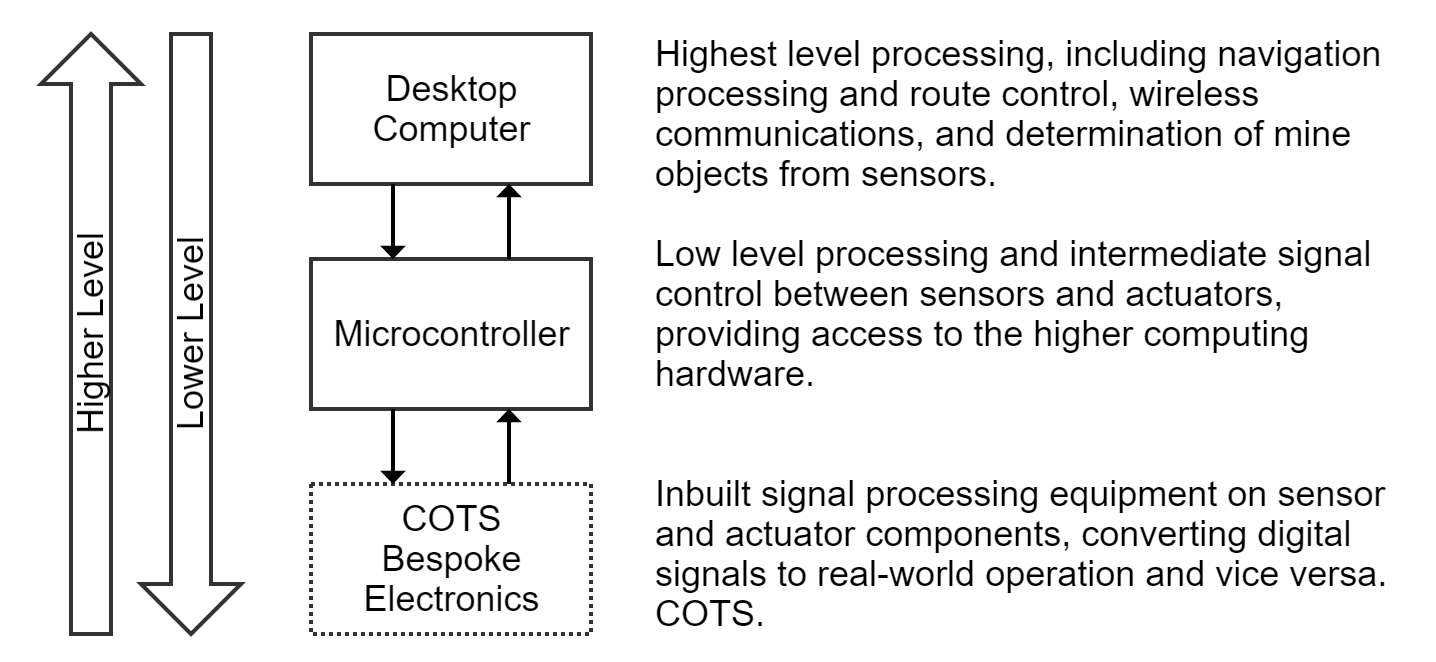
\includegraphics[width = \textwidth]{4-ConceptDesign/electronics.png}
\centering
\caption{Conceptual Hardware layout} \figlabel{hardwareLayout}
\end{figure}

Under this system, the project will use standard desktop computing equipment for the bulk of the software, to make use of its superior processing power and the rapid development it allows. This device will be the data handler and processor, and act as the 'central' software location for the project. Sensors and actuators that require low level I/O access will be connected to a secondary microcontroller, which will act independently to buffer inputs and outputs of the system, which can then be communicated to the primary computer over a serial communications connection. The project will not aim to develop any custom electronics boards and handle all signal amplification or processing in software.

\section{Sensor Mount}

\section{Conceptual Project Design}
\textcolor{green}{CONCEPTUAL DESIGN SHOULD FINISH WITH A DESIGN. WHERE IS IT? <-- straight from the maz's mouth. Need some top level diagrams, flowcharts and shit down here to tie together the entire project}

\end{document}